\documentclass[12pt]{article}
\usepackage{amsmath}
\usepackage{multicol}
\usepackage{amssymb}
\usepackage{bbding}
\usepackage{pifont}
\usepackage{wasysym}
\usepackage{amssymb}
 \usepackage{graphicx}
 \usepackage{wrapfig}
 \usepackage{float}
 \usepackage{calc}
\usepackage{eso-pic}
\usepackage{tikz}

\newlength{\PageFrameTopMargin}
\newlength{\PageFrameBottomMargin}
\newlength{\PageFrameLeftMargin}
\newlength{\PageFrameRightMargin}

\setlength{\PageFrameTopMargin}{1cm}
\setlength{\PageFrameBottomMargin}{1cm}
\setlength{\PageFrameLeftMargin}{1cm}
\setlength{\PageFrameRightMargin}{1cm}

\makeatletter

\newlength{\Page@FrameHeight}
\newlength{\Page@FrameWidth}

\AddToShipoutPicture{
  \thinlines
  \setlength{\Page@FrameHeight}{\paperheight-\PageFrameTopMargin-\PageFrameBottomMargin}
  \setlength{\Page@FrameWidth}{\paperwidth-\PageFrameLeftMargin-\PageFrameRightMargin}
  \put(\strip@pt\PageFrameLeftMargin,\strip@pt\PageFrameTopMargin){
    \framebox(\strip@pt\Page@FrameWidth, \strip@pt\Page@FrameHeight){}}}

\makeatother
\begin{document}
\title{Domain of Linear Algebra}
\author{Khush Thakor}
\date{11/18/2022}
\makeatletter
\renewcommand*\env@matrix[1][*\c@MaxMatrixCols c]{%
  \hskip -\arraycolsep
  \let\@ifnextchar\new@ifnextchar
  \array{#1}}
  \renewcommand*\contentsname{Table of Contents}
\makeatother
\maketitle
\begin{center}
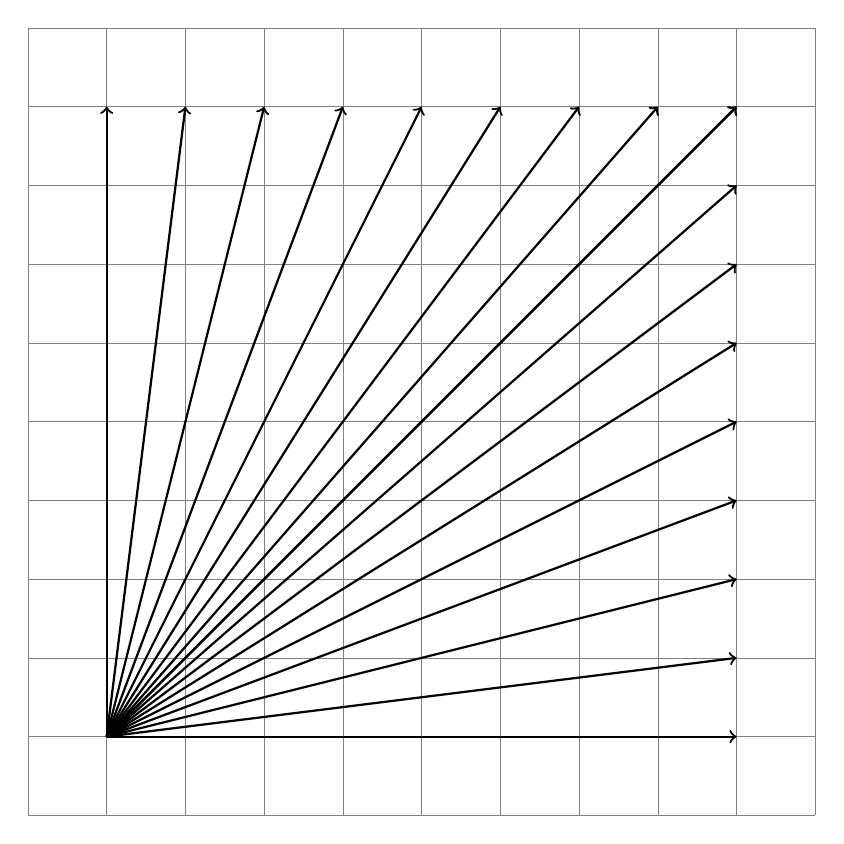
\begin{tikzpicture}
\draw[step=1cm,gray,very thin] grid(10,10);
\draw[thick,->] (1,1) -- (9,1);
\draw[thick,->] (1,1) -- (1,9);
\draw[thick,->] (1,1) -- (9,2);
\draw[thick,->] (1,1) -- (2,9);
\draw[thick,->] (1,1) -- (9,3);
\draw[thick,->] (1,1) -- (3,9);
\draw[thick,->] (1,1) -- (9,4);
\draw[thick,->] (1,1) -- (4,9);
\draw[thick,->] (1,1) -- (9,5);
\draw[thick,->] (1,1) -- (5,9);
\draw[thick,->] (1,1) -- (9,6);
\draw[thick,->] (1,1) -- (6,9);
\draw[thick,->] (1,1) -- (9,7);
\draw[thick,->] (1,1) -- (7,9);
\draw[thick,->] (1,1) -- (9,8);
\draw[thick,->] (1,1) -- (8,9);
\draw[thick,->] (1,1) -- (9,9);
\draw[thick,->] (1,1) -- (9,9);
\end{tikzpicture}
\end{center}
\newpage
\tableofcontents
\section*{Introduction}
\textbf{Linear Algebra} is an extensive mathematical course which investigates fundamental properties of abstract spaces such as vector spaces. It takes a look at the way to represent linear transformations using matrices. Matrix properties are also an essential property which affect all concepts involving Linear Algebra. Linear Algebra is only the foundation to many mathematical concepts to come such as Differential Equations. As you go through you will also see Linear Algebra has a magnitude of application in other science like Chemistry. However one of the biggest applications is Computer Science where the use of matrices to store information is crucial in a such data related field. This guide is a way to introduce you to the essentials you may encounter in a college Linear Algebra course.
\\\\
This book was crafted from various portfolios I wrote while studying Linear Algebra at Pierce College. Special Acknowledgment to Dr. Erica Shannon and Pierce College Mathematics Department for inspiration to crafting this project, as well help with review of book. Format of this books is crafted using \LaTeX and using TeXworks to compile code. The source code can be found at https://github.com/khush-Thakor/DomainOfLinearAlgebra
\newpage
\section*{Format}
Throughout this book I present problems at the beginning of each section which cover all the content through the concept. This book was For example\\\\
\fbox{Solve the Liner System of Equations}
\begin{equation*}x_1+2x_2=5
\end{equation*}
\begin{equation*}2x_1+5x_2=7
\end{equation*}
\fbox{Liner System of Equations}\\\\
For this problem we must use our knowledge of matrices and how we can represent a linear system in a augmented matrix.
\\\\ \textbf{Linear System representation in a Matrix}
\begin{equation*}
A = \begin{bmatrix}[c c| c]
1 & 2 & 5 \\
2 & 5 & 7
\end{bmatrix}
\end{equation*}
\\\\ \textbf{Reduced Row Echelon Form of $A$}
\begin{equation*}
\text{rref}(A) = \begin{bmatrix}[c c| c]
1 & 0 & 1 \\
0 & 1 & -3
\end{bmatrix}
\end{equation*}
\\\\
An explanation of the given topic or subtopic will be provided in this section. A general solution that we can take the problem will also presented. Terms through the book will be used however definition and examples will also be provided. Most problems invoke questions about the given topic at hand. By \\\\
\fbox{Reflection Liner System of Equations}\\\\
At the end of each chapter or sub section a reflection is provided which would relay all the information for a generic problem of the sub topics.
\begin{center}
\newpage
\section*{About the Author}
    \includegraphics[width=50mm]{profilePic}
\end{center}
\par
\begin{multicols}{2}
I am Khush Thakor a high school senior studying computer science at Pierce College. I work as a Supplemental Instructor for CS 141 and CS 202 (Data Structures and Algorithms) at Pierce College and hold responsibilities for District Tech Lead at Pierce College Peer Academic Support Services. I am peer tutor in Computer Science, Calculus (I-III), Linear Algebra, and Calculus-based Physics. I am recently active as the President of the Society of Physics Students at Pierce College and a lead contributor to a dc discharge plasma research experiment. When not learning computer science, I run cross country, swim on the varsity swim team, and hike the pacific northwest. I can be contacted at khushthakor@gmail.com.
\end{multicols}
\pagebreak
\pagebreak
\section{Linear Systems}
\makeatother
\subsection{Solution to a Linear System}
We will be taking a look at the process of finding the \textbf{solution} to a linear system using matrices\\\\
\fbox{Example}
\bigskip
\begin{align*}
2x+3y=4 \\
-3x+4y=11 
\end{align*}
\medskip
\\We can look at the linear systems as a matrix multiplication problem. Next step is to turn our system in a matrix form. \\
\bigskip
\newline
A = $\begin{bmatrix}
  2 & 3 \\
  -3 & 4
\end{bmatrix}$, $\vec{x}=$ $\begin{bmatrix} 
  x \\
  y
\end{bmatrix}$, $\vec{b} =$ $\begin{bmatrix}
  4 \\
  11
\end{bmatrix}$
\\\\ The matrix $A$ is achieved from the $x$ and $y$ values from our 2 equations in our system. Each of the equation has it sown row and each column represents the $x$ or $y$ values .
\newline
\\
Now we can use the form $$A\vec{x} = \vec{b}$$
and solve for $\vec{x}$. We can achieve this by taking the inverse of $A$ and multiplying $A^{-1}$ on both sides of our equation.
\begin{equation*}
AA^{-1}=I
\end{equation*}
\\Where $I$ will be the identity matrix.
\\\\ \fbox{Example of Identity Matrix of 2 x 2}
\begin{equation*}
I = \begin{bmatrix}1 & 0 \\ 0 & 1\end{bmatrix}
\end{equation*}
 We can only take the inverse if our matrix is invertible, meaning that it does have the same number of rows and columns and the determinant is not 0. If the matrix $A$ is not invertible we have to set up an augmented matrix and solve by obtaining the reduced row echelon form. 
\\ Here is the augmented matrix we could use.
\[\begin{bmatrix}[cc|c]
2 & 3 & 4\\
-3 & 4 & 11
\end{bmatrix}
\]
We know that we can solve for $\vec{x}$ using the inverse because $A$ is a square matrix, meaning has same number of rows nad columns and the determinant is not equal to 0. Now we can apply 
\begin{equation*}
A^{-1}A=I 
\end{equation*}
to write that
\begin{equation*}
\vec{x}=A^{-1} \vec{b}
\end{equation*}
The following step would be to solve for the inverse of A. We can achieve this by using the formula for a 2x2 matrix inverse
\begin{equation*}
A = \begin{bmatrix}
  a & b \\
  c & d
\end{bmatrix}\\\\
\end{equation*}
\begin{equation*}
A^{-1}=\frac{1}{\text{det}(A)}\begin{bmatrix}
  d & -b \\
  -c & a
\end{bmatrix}
\end{equation*}
Our det(A) being our determinant which we can find by 
$\text{det}(A)\ = (ad) - (bc)$\\
Steps to solution
\begin{equation*}
  \begin{bmatrix}
    2 & 3 \\
    -3 & 4
  \end{bmatrix} \begin{bmatrix}
    x \\
    y
  \end{bmatrix}
  = \begin{bmatrix}
    4 \\
    11
  \end{bmatrix} \\
  \end{equation*}
  \begin{equation*}
17 = \text{det}(A)\ = (2\times 4) - (-3\times 3)
\end{equation*}
\begin{equation*}
A^{-1} = \begin{bmatrix}
\frac{4}{17} \frac{-3}{17} \\
\frac{3}{17} \frac{2}{17} \\
\end{bmatrix}
\end{equation*}
\begin{equation*}
\begin{bmatrix}
\frac{4}{17} & \frac{-3}{17} \\
\frac{3}{17} & \frac{2}{17} \\
\end{bmatrix}
\begin{bmatrix}
4 \\ 11
\end{bmatrix} = \begin{bmatrix}
-1 \\ 2
\end{bmatrix}
\end{equation*}
After multiplying our inverse with our vector we now have a vector $\vec{x}$ such that $A\vec{x} =\vec{b}$. This shows how we can solve for a $\vec{x}$ using inverses knowing matrix $A$ and vector $\vec{b}$.
\\\\ \fbox{Reflection of Systems}\\
\begin{flushleft}
When we want to solve a system of equations with matrices, we can use inverses to form a solution. First we can identify our matrix of coefficients from the system. This will allow us to get all the $x$ and $y$ values then find a vector for our solution. Thinking of the problem as 1 matrix, $ A \text{ and 2 vectors }\vec{b}$ and  $\vec{x}$ where $A \vec{x} = \vec{b}$. When our matrix A is invertible we can take the inverse of $A$ and multiply it on both sides inorder to get our identity matrix on the left side, now we have the form of $\vec{x} = A^{-1}\vec{b}$. This shows how to find the determinant of a matrix using non technology methods and solve a system.
\end{flushleft}
\subsection{Chemical Equations and Linear Algebra}
Balance the following Chemical Equation
\begin{equation*}
\text{Fe}+\text{O}_2 \rightarrow \text{Fe}_2\text{O}_3
\end{equation*}
In order for us to balance the equation we have to write the coefficients
\begin{equation*}
x_1\text{Fe}+x_2\text{O}_2 \rightarrow x_3\text{Fe}_2\text{O}_3
\end{equation*}
We can write a system of equation for the elements.
\begin{equation*}
x_1+0x_2=2x_3 \\
0x_1+2x_2=3x_3
\end{equation*} 
We can put all of our variables on one side in order to to turn our equation into a matrix. In our case we have two elements Fe and O therefore we will have 2 rows and 4 columns.  Having the matrix columns for the coefficients for $x_1, x_2, x_3$.
\begin{equation*}
A = \begin{bmatrix}[ccc|c]
1 & 0 & -2 & 0\\
0 & 2 & -3 & 0\\
\end{bmatrix}
\end{equation*}
The next step would be to turn our matrix into row reduced echelon form. We can achieve this by applying row operations in order to eliminate rows.
In this matrix we only need one step to achieve row reduced form and that is to subtract the 2nd row with a 1/2 multiply of the 2nd row
\begin{equation*}
r_{2} = r_2 - \frac{r_{2}}{2}
\end{equation*}
Which would give the row reduced form of the Matrix
\begin{equation*}
  A = \begin{bmatrix}[ccc|c]
  1 & 0 & -2 & 0\\
  0 & 1 & -1.5 & 0\\
  \end{bmatrix}
  \end{equation*}
 After obtaining the row reduced form of the Matrix we can create our solution set for the Chemical Equation
 \begin{equation*}
 x_1 = 2x_3 \\
 x_2 = 1.5x_3 \\
 x_3 = x_3
 \end{equation*}
 We notice that $x_3$ has a coefficient of 1.5. We have the smallest of value of $x_3$ for it to create a whole number. We can say $x_3=2$ that would result in $x_2=3$ and $x_1=4$
  \begin{equation*}
 x_1 = 4 \\
 x_2 = 2 \\
 x_3 = 2
 \end{equation*}
 Finally we apply our values back to our chemical equation and get our balanced equation
 \begin{equation*}
4\text{Fe}+3\text{O}_2 \rightarrow 2\text{Fe}_2\text{O}_3
\end{equation*}\\
\fbox{Reflection for Chemical Equations}\\\\
For a problem that asks to balance a chemical equation using system of equations, the best way to approach the problem is to first organize the elements given to you. Then list all the coefficients you can make with the equation. After that one by one for the elements create the linear equations. After establishing the linear equations we have then get the system into reduced row echelon form using Gaussian Elimination. This will be a critical step into finding the solution to the linear system. Next step is to create the solution set from the reduced row echelon matrix. Critical information that we need in the problems is the number of elements and moles of each element given in the equation. Keeping track of the coefficients and variables created is also crucial to successful solving the problem. This problem shows applying linear systems to topics outside of Linear Algebra like chemistry in which we are able to use linear systems to balance chemical equations. Also showing the understanding of Gaussian Elimination in order to obtain the row reduced from of a matrix.
\newpage
\section{Introduction to Matrices}
\subsection{Transpose of Matrix}
We are given a matrix $A$. Find $A^{T}$, rref$(A)$. Then find the \textbf{rank}, \textbf{invertibility}, and \textbf{determinant}
\begin{align*}
A = \begin{bmatrix}
  1 & 2 & 2 & 26 \\
  0 & 1 & 1 & 12 \\
 0 & 0 & 1 & 9 \\
\end{bmatrix}
\end{align*}
\medskip
\newline
In order to find the transpose of an matrix we much switch the rows and columns of the matrix. General form of the transpose of a matrix is
\begin{align*}
A = \begin{bmatrix}
  x_{1} & x_{2} & x_{3} \\
  x_{4} & x_{5} & x_{6} \\
  x_{7} & x_{8} & x_{9}
\end{bmatrix}
\\
A^{T} = \begin{bmatrix}
  x_{1} & x_{4} & x_{7} \\
  x_{2} & x_{5} & x_{8} \\
  x_{3} & x_{6} & x_{9}
\end{bmatrix}
\end{align*}
Now we can use this approach to our 3 x 4 Matrix.
\begin{align*}
A = \begin{bmatrix}
  1 & 2 & 2 & 26 \\
  0 & 1 & 1 & 12 \\
 0 & 0 & 1 & 9 \\
\end{bmatrix}
\rightarrow
A^{T} = \begin{bmatrix}
 1 & 0 & 0  \\
 2 & 1 & 0  \\
 2 & 1 & 1  \\
 26 & 12 & 9  \\
 \end{bmatrix}
\end{align*}
\\ Notice our 3 x 4 matrix turned into a 4 x 3 matrix. Our number of rows and columns switched. In a square matrix they would remain the same. \\\\
\subsection{Reduced Row Echelon Form}
To find the \textbf{reduced row echelon form} of the matrix we can do row operations.
First we have to reduce the 2nd row by subtracting the 3rd row from the 2nd row
\begin{align*}
A = \begin{bmatrix}
 1 & 2 & 2 & 26 \\
  0 & 1 & 0 & 3 \\
 0 & 0 & 1 & 9 \\
 \end{bmatrix}
\end{align*}
Next we can reduce the first row by subtracting the 2nd row multiplied by a factor 2
\begin{align*}
A = \begin{bmatrix}
 1 & 0 & 2 & 20 \\
  0 & 1 & 0 & 3 \\
 0 & 0 & 1 & 9 \\
 \end{bmatrix}
\end{align*}
Lastly we can reduce the first row by subtracting twice the 3rd row
\begin{align*}
A = \begin{bmatrix}
 1 & 0 & 0 & 2 \\
  0 & 1 & 0 & 3 \\
 0 & 0 & 1 & 9 \\
 \end{bmatrix}
\end{align*}
Getting our \textbf{reduced row echelon form}. We know that we have a reduced row echelon form when 
\begin{itemize}
  \item Non zero rows are above all zeroes (if any)
  \item Each left most entry (leading entry) is in a column to the right of the previous leading entry
  \item All leading entries are 1
   \item All entries above a leading entry are 0
\end{itemize}
\begin{align*}
\text{rref}(A) = \begin{bmatrix}
 1 & 0 & 0 & 2 \\
  0 & 1 & 0 & 3 \\
 0 & 0 & 1 & 9 \\
 \end{bmatrix}
\end{align*}
Our matrix is now in reduced row echelon form because it meets all requirements of reduced row echelon form.
Once we have our reduced row echelon form, we can determine our rank. The rank is the number of nonzero rows in the reduced row echelon matrix and in our case the \textbf{rank} is 3.
\newline
\subsection{Matrix Operations}
To find the \textbf{invertibility} we have to know if the matrix is invertible or not. A matrix is invertible if it is a square matrix meaning it has same number of rows and columns and it has a nonzero determinant. We have a 3 x 4 matrix which \textbf{is not} invertible since it does not have the same number of rows and columns.
\newline
\begin{align*}
A = \begin{bmatrix}
  1 & 2 & 2 & 26 \\
  0 & 1 & 1 & 12 \\
 0 & 0 & 1 & 9 \\
\end{bmatrix}
\bigskip
\end{align*}
If we were given a matrix $C = \begin{bmatrix}1 & 4 \\ 3 & 5\end{bmatrix}$. Then we can find $C^-1$ (inverse of C) with the following formula
\begin{equation*}C = \begin{bmatrix}x_1 & x_2 \\ x_3 & x_4\end{bmatrix}\end{equation*}
\begin{equation*}C^{-1} = \begin{bmatrix}\frac{x_4}{\text{det}(C)} & \frac{x_1}{\text{det}(C)}\\ \frac{-x_3}{\text{det}(C)} & \frac{-x_4}{\text{det}(C)}\end{bmatrix}\end{equation*}
\begin{equation*}C^{-1}= \begin{bmatrix}\frac{-5}{7} & \frac{4}{7}\\ \frac{3}{7} & \frac{-1}{7}\end{bmatrix}\end{equation*}
If we were given a matrix $B$ = 
 $\begin{bmatrix}
 1 & 1 & 1 & 2 \\
  3 & 1 & 0 & 2 \\
 0 & 1 & 1 & 3 \\
 \end{bmatrix}$
 We can find A + B by adding the matrices
 \begin{align*}
A +B = \begin{bmatrix}
 1+1 & 2+1 & 2+1 & 26+2 \\
  0+3 & 1+1 & 1+0 & 2+12 \\
 0+0 & 0+1 & 1+1 & 9+3 \\
 \end{bmatrix}
 \end{align*}
  \begin{align*}
A +B = \begin{bmatrix}
 2 & 3 & 3 & 28 \\
  3 & 2 & 1 & 14 \\
 0& 1 & 2 & 12 \\
 \end{bmatrix}
  \end{align*}
  \\\\ We can scale a matrix as well by also scaling each component.
  \begin{equation*}2A = \begin{bmatrix}2& 4 &4 &52 \\ 
  0& 2 &2 &24 \\
  0& 0 &2 &18 \\
  \end{bmatrix}\end{equation*}
We can do similar operations with subtraction by subtracting all the components
\begin{align*}
  A -B = \begin{bmatrix}
 1-1 & 2-1 & 2-1 & 26-2 \\
  0-3 & 1-1 & 1-0 & 12-2 \\
 0-0 & 0-1 & 1-1 & 9-3 \\
 \end{bmatrix}
 \end{align*}
  \begin{align*}
  A -B = \begin{bmatrix}
 0 & 1 &1 & 24 \\
  -3 & 0 & 1 & 10 \\
 0& -1 & 0 & 6 \\
 \end{bmatrix}
\end{align*}\\
\fbox{Matrix Operations Reflection}\\
\begin{flushleft}
When approaching row reduction problems we can take the strategy of eliminating the rows by adding subtracting, or multiplying factors of other rows in order to get the matrix into reduced row echelon form. Critical components are writing out step by step of the elimination of rows. This problems shows the understanding of the properties of a matrix as well as the demonstration of the row reduction of the matrix. This example showing the how to use matrix operations of adding and subtracting matrices.
\end{flushleft}
\newpage
\section{Determinant of Matrix}
\subsection{The Determinant}
Given a matrix $A$, Find the determinant of the given matrix.
\newline
\begin{align*}
A = \begin{bmatrix}
  1 & 3 & 4 \\
  0 & 1 &2 \\
 0 & 1 & 3 \\
\end{bmatrix}
\end{align*}
We can find the determinant of a matrix by expanding along a row or a column. The expansion along the top row in order to find the determinant can be shown like
\begin{align*}
A = \begin{bmatrix}
x_{1} & x_{2} & x_{3} \\
  x_{4} & x_{5} & x_{6} \\
  x_{7} & x_{8} & x_{9}
\end{bmatrix}
\end{align*}
\begin{align*}
\text{det}(A) = x_{1} (x_{5}x_{9}-x_{8}x_{6})-x_{2} (x_{4}x_{9}-x_{7}x_{6})+x_{3} (x_{4}x_{8}-x_{5}x_{7})
\end{align*}
Now we can apply this to our problem in which we can expand along the top row of our matrix
\begin{align*}
\text{det}(A) = 1(1(3)-1(2))-3(0(3)-0(2))+4(0(1)-0(1))
\end{align*}
We can get our determinant to be
\begin{align*}
det(A) = 1
\end{align*}
\fbox{Reflection on Determinants}
\begin{flushleft}
When approaching a problem that asks for the determinant of a matrix we can expand along any row or column of the matrix. For problems it is best practice to write out the matrix and then write out our form in which we expand along the row or column. In the problem above I expanded along the top row however we can do it to any row or column. Key information to note is the organization of the steps used to expand and then the correctly simplifying afterward to get the correct answer as well. Not keeping track of numbers and the expansion  along a row or column can lead to skipping steps or miscalculation which will result in a wrong determinant.
\end{flushleft}
\newpage
\section{Vector Spaces}
Let $V =  \mathbb{R}^3$ and let $\left\{S = \begin{bmatrix}x \\ y \\ z \end{bmatrix} \in V : y\geq x \text{ and } z = 0 \right\}$ Is $S$ a subspace of $V$? Justify your answer.
\\\\
For this question we have to investigate the definition of a subspace and conduct the subspace test. We know that a space is a subspace if and only if passes the \textbf{subspace test}. \\\\
\fbox{Definition of Vector Space}\\\\
A vector space is a set of vectors with two operations defined addition and scalar multiplication, which satisfy the axioms of addition and scalar multiplication.
\\\\ \textbf{Axioms of Addition}
\\\\Consider $\vec{v}, \vec{z}, \vec{w} \in V$
\\ \begin{enumerate}
  \item $\vec{v}+ \vec{w} \in V$ (Closed under addition)
  \item $\vec{v}+ \vec{w} = \vec{w}+ \vec{v}$ (Commutative)
  \item $(\vec{v}+ \vec{w}) + \vec{z} = (\vec{z}+ \vec{w}) + \vec{v}$ (Associative)
  \item $(\vec{w} + \vec{0} = \vec{w})$ (Additive Identity)
  \item $(\vec{w} + -\vec{w})= 0$ (Additive Identity Inverse)
  \end{enumerate}
\textbf{Axioms of Scalar Multiplication}
\\\\Consider $\vec{v}\in V$ and $ a \in \mathbb{R}^2$
\\ \begin{enumerate}
  \item $a\vec{v} \in V$ (Closed under Scalar Multiplication)
  \item $a\vec{v}+ a\vec{w} = a(\vec{v}+ \vec{w})$ (Distrubution Scalar Multiplication)
  \item $(b(a\vec{v}) = (ba)(\vec{v})$ (Associative)
  \item $(1\vec{v} = \vec{v})$ (Scalar Identity)
  \end{enumerate}
  Following the Axioms of Addition and Axioms of Scalar Multiplication we can create 2 vectors
  \begin{equation*}
    \vec{v} = \begin{bmatrix}x_1 \\ y_1 \\ z_1\end{bmatrix} \text{and } \vec{w} = \begin{bmatrix}x_2 \\ y_2 \\ z_2 \end{bmatrix}
  \end{equation*}
  where $\vec{v} \in \mathbb{R}^3$ and $\vec{w}\in \mathbb{R}^3$.
  \\\\We can show that $\mathbb{R}^3$ is a vector space.
  \\ \begin{enumerate}
    \item $\vec{v}+ \vec{w} \in \mathbb{R}^3$ (Closed under addition) \checkmark
    \item $\vec{v}+ \vec{w} = \vec{v}+ \vec{w}$ (Commutative) \checkmark
    \item $\vec{z} \in \mathbb{R}^3, (\vec{v}+ \vec{w}) + \vec{z} = (\vec{v}+ \vec{w}) + \vec{z}$ (Associative) \checkmark
    \item $(\vec{v} + 0 = \vec{v})$ (Additive Identity) \checkmark
    \item $(\vec{v} + -\vec{v})= 0$ (Additive Identity Inverse) \checkmark
    \end{enumerate}
\fbox{Axioms of Sclar Multiplation}
  \begin{enumerate}
    \item $c \in \mathbb{R},c\vec{v} \in \mathbb{R}^3$ (Closed under Scalar Multiplication) \checkmark
    \item $c \in \mathbb{R},c\vec{v}+ c\vec{w} = c(\vec{v}+ \vec{w})$ (Dsitrubution Scalar Multiplication) \checkmark
    \item $c \in \mathbb{R},b \in \mathbb{R},(b(c\vec{v}) = (bc)(\vec{v})$ (Associative) \checkmark
    \item $(1\vec{v} = \vec{v})$ (Additive Identity)\checkmark
    \end{enumerate}
    We can say that $\mathbb{R}^3$ is a vector space \\\\
    \subsection{Subspaces}
\fbox{Subspace Test} \\\\
Suppose we have $W$ which is a subset of $V$. $W$ is a subspace of V if it passes all three rules
\\ \begin{enumerate}
  \item $\vec{0} \in	 W$ (Subspace must contain Zero Vector)
  \item For any $w_1 \in W$ and $w_2 \in W$, $\vec{w_1}+ \vec{w_2} \in W$ (Subspace must be closed under addition)
  \item For any $a\in \mathbb{R}$ and $w_1 \in W$, $\vec{aw_1}\in W$ (Subspace must be closed under scalar multiplication)
\end{enumerate}
Using our steps for the subspace test we can determine whether $S$ is a subspace of $V$.\\\\
Remember \\
$V =  \mathbb{R}^3$ and let $ \{S = \begin{bmatrix}x \\ y \\ z \end{bmatrix} \in V : y\geq x$ and $ z = 0\}$
\\ \begin{enumerate}
  \item $\vec{0} \in S$ ($S$ contains Zero Vector) \checkmark
  \item For any $\vec{w_1} \in S, \vec{w_2} \in S, \vec{w_1}+ \vec{w_2} \in S$ (Subspace is closed under addition) \checkmark
  \item For any $a\in \mathbb{R}$ and $\vec{w_1}\in S$ $aw_1 \notin S$ (Subspace is \textbf{NOT} closed under scalar multiplication)
\end{enumerate}
\begin{equation*}
\begin{bmatrix}
0 \\ 0 \\ 0
\end{bmatrix} \in S 
\end{equation*}
\begin{center}Contains $\vec{0}$
\\
\begin{equation*}
\begin{bmatrix}
x_1 \\ y_1 \\ 0
\end{bmatrix} + \begin{bmatrix}
x_2 \\ y_2 \\ 0
\end{bmatrix} = \begin{bmatrix}
x_1+x_2 \\ y_1+y_2 \\ 0
\end{bmatrix} \in S
\end{equation*}
If $y_1 \geq x_1 $ and $y_2 \geq x_2$ then $y_1+y_2 \geq x_1+x_2$\\
Closed under Addition \\
\end{center}
\begin{center}
\begin{equation*}
-a\begin{bmatrix}
x_1 \\ y_1 \\ z_1
\end{bmatrix}= \begin{bmatrix}
ax_1 \\ ay_1 \\0
\end{bmatrix} \notin S
\end{equation*}
If $a \ge 0,  y_1 \geq x_1 $ then $-ay_1\leq -ax_1$\\
Not closed under scalar multiplication
\end{center}
We can see that $S$ is closed under vector addition and contains the zero vector. However the space is not closed under scalar multiplication. If we do multiply a negative scalar to a vector in the space we do get a vector that is not in $S$ since $y\geq x$ and a larger negative $y$ would be less than a smaller negative $ x$, therefore the vector would not be be in $S$.
We can conclude that $S$ is not a subspace of $V$ because it does not pass all steps of the subspace test.
\subsection{Matrix Properties}
Given that $A = \begin{bmatrix}5 & 1 & 0 \\ 3 & 4 & 0 \\ 2 & 3 &1 \end{bmatrix}$
\\\\ Find the dimension and basis for the column space, nullspace and row space. \\\\
In order to find the column space of the matrix we must first find the rank and we can do this by taking the rref of $A$
\begin{equation*}
rref(A) = \begin{bmatrix}1 & 0 & 0 \\ 0 & 1 & 0 \\ 0 & 0 &1 \end{bmatrix}
\end{equation*}
\subsection{Column Space}
We can see by this the rank will be 3. The dimension of the column space will be 3 since it is the same as the rank. Since our dimension is 3 we get a column space of all $\mathbb{R}^3$. We can form a basis to be
\begin{equation*}\left\{\begin{bmatrix}1 \\ 0 \\ 0  \end{bmatrix},\begin{bmatrix}0 \\ 1 \\ 0  \end{bmatrix},\begin{bmatrix} 0 \\ 0 \\ 1  \end{bmatrix}\right\}\end{equation*}
\subsection{Null Space}
In order to find the nullspace for our matrix we can solve it as we are solving a homogeneous system by turning the matrix into an augmented matrix augmented with the zero vector
\begin{equation*}
\begin{bmatrix}[ccc|c]
5 & 1 & 4 & 0\\
3 & 4 & 0 & 0\\
2 & 3 & 1 & 0 \\
\end{bmatrix}
\rightarrow
rref(A) = \begin{bmatrix}[ccc|c]
1 & 0 & 0 & 0\\
0 & 1 & 0 & 0\\
0 & 0 & 1 & 0 \\
\end{bmatrix}
\end{equation*}
We can see from the reduced row echelon form that we get a 0 dimensional nullspace at the point at 
\begin{equation*}
\begin{bmatrix}
 0\\
 0\\
 0 \\
\end{bmatrix}
\end{equation*}
Since the nullspace is the 0 vector we cannot create a basis.
\\\\ Now to find the row space we have to find the basis of all the row vectors. The dimension of the row space is the same as the rank. Which will also be 3, therefore we can get the basis to also be
\begin{equation*}\left\{\begin{bmatrix}1 \\ 0 \\ 0  \end{bmatrix},\begin{bmatrix}0 \\ 1 \\ 0  \end{bmatrix},\begin{bmatrix}0 \\ 0 \\ 1  \end{bmatrix}\right\}\end{equation*}
\fbox{Vector Spaces and Subspace Reflection} \\\\
In Problem 1 we are asked to find if a given space is subspace of a vector space. For these problems we must use the subspace test and all of the steps that are listed in the definition above. Going through each step such as finding if the 0 vector exists in our space is crucial because all we need is one case where the test fails and we will not have a subspace. We also do need to make sure that when checking for closed under addition and scalar multiplication we need to check all cases such as positive and negative scalars because those can also have a different affect on the vector and our set may not be a subspace then.
\\\\In problem we were asked to find the column space, nullspace and row space of a given matrix. Crucial information that is need to find these spaces is that we needed the rank of the matrix. Dimensions of row and column space can be figured out using the rank and in that we can also take a look at how the space will look being that 0 dimensional is a point, 1 dimension is a line and 2 is plane and moving further with more dimensions. We can then find the nullspace by making the matrix augmented with the zero vector to also get the dimensions of the nullspace. When finding a basis for the spaces if we have spaces such as all of $\mathbb{R}^2$ we can just use the standard basis vector to form a basis for the given space.
\newpage
\section{Basis of Vector Space}
Consider the vectors $\vec{v_1}, \vec{v_2}, \vec{v_3}$ where \\\\
$\vec{v_1} = \begin{bmatrix} 1 \\ 2 \\ 1\end{bmatrix}$,
$\vec{v_2} = \begin{bmatrix} 3 \\ 1 \\ 4\end{bmatrix}$,
$\vec{v_3} = \begin{bmatrix} 1 \\ 1 \\ -1\end{bmatrix}$
\\\\Determine if  $v_1, v_2, v_3$ are linearly independent. Compute span$\{\vec{v_1}, \vec{v_2}, \vec{v_3}\}$
\subsection{Linear Independence}
A set of of nonzero vectors $\{\vec{w_1}, \vec{w_1},..,\vec{w_n}\}$ is \textbf{linearly independent} if the only way to have
\begin{equation*}a_1\vec{w_1}+a_2\vec{w_2}+...+a_m\vec{w_m} = \vec{0}\end{equation*}
is to have all the coefficients of $a_i=0$
\\\\ Applying this to our problem we can say that $v_1, v_2, v_3$ are linearly independent if
\begin{equation*}
a_1 \begin{bmatrix} 1 \\ 2 \\ 1\end{bmatrix}
a_2  \begin{bmatrix} 3 \\ 1 \\ 4\end{bmatrix}
a_3 \begin{bmatrix} 1 \\ 1 \\ -1\end{bmatrix} = 0
\end{equation*}
we can also write this an augmented matrix, where our columns are our vectors and we can augment them to the zero vector. We can then take turn our matrix into reduced row echelon form to see if we can get an values of  $a$ which can make a linear combinations of the vectors to get the zero vector.
\begin{equation*}
A = 
 \begin{bmatrix}[ccc|c] 
 1 & 2 & 1 & 0 \\
 3 & 1 & 4 & 0 \\
1 & 1 & -1 & 0 
\end{bmatrix}
\end{equation*}
\begin{equation*}
\text{rref}(A) = 
 \begin{bmatrix}[ccc|c] 
 1 & 0 & 0 & 0 \\
 0 & 1 & 0 & 0 \\
0 & 0 &  1 & 0 
\end{bmatrix}
\end{equation*}
Our reduced row echelon matrix tells us that all scalars $a_1, a_2, a_3$ have to be 0 inorder our vectors be a linear combination that equals the zero vector. This tells use that $\{\vec{v_1}, \vec{v_2}, \vec{v_3}\}$ are a set of linearly independent vectors.
\subsection{Span}
In order to determine the span of the vectors we can take a look at the rank of the matrix where the vectors are the columns. We can see that the rank is 3, which is the dimension of our span of vectors. Having a span of 3 dimensions would make the span all of $\mathbb{R}^3$
\begin{equation*}\text{span}\{\vec{v_1}, \vec{v_2}, \vec{v_3}\} = \mathbb{R}^3\end{equation*}
\fbox{Reflection for Linear Independence and Span}\\\\
This problem asks about determining if a set of vectors is linearly independent and asks what is the span of the given vector space. Crucial information is the vector set that is given because then we create augmented matrix to determine if the given vectors are linearly independent. It is important that we correctly set up our augmented matrix with columns of all the vectors augmented to the zero vector because if we incorrectly augment our matrix we may get a reduced row echelon which gives incorrect scalars for linear combinations. This artifact shows my ability to determine whether or not a given subset of a vector space is linearly independent and compute the span of a given subset of a vector space.
\subsection{Basis}
Determine whether the set of vectors  $ W = \left\{\begin{bmatrix}2 \\ 3\end{bmatrix},\begin{bmatrix}8 \\ 12\end{bmatrix}\right\}$ is a basis for $\mathbb{R}^2$
\fbox{Definition of Basis}\\\\
Consider that a subset $W = \{\vec{w_1},\vec{w_2},...,\vec{w_n}\}$ is a subspace of the vector space $V$.
\\\\ We can say that $W$ is a basis for $V$ if 
\begin{itemize}
  \item $W$ is linearly independent
  \item $W$ spans $V$
\end{itemize}
Therefore in our question $W$ has to be linearly independent and span $\mathbb{R}^2$ in order to say that $W$ is a basis for $\mathbb{R}^2$
\\\\ We can set up an augmented matrix with our columns being the vectors of $W$ to determine if $W$ is linearly independent and if $W$ can span all of $\mathbb{R}^2$
\begin{equation*}
A = 
 \begin{bmatrix}[cc|c] 
2 & 8 & 0 \\
3 & 12 &0
\end{bmatrix}
\end{equation*}
\begin{equation*}
\text{rref}(A) = 
 \begin{bmatrix}[cc|c] 
 1 & 4 & 0\\
 0 & 0 & 0\\
\end{bmatrix}
\end{equation*}
We can see that from our reduced row echelon matrix that we have rank of 1, which would mean that our span of vectors is only 1 dimensional. The vectors are also not linearly independent because we can write
\begin{equation*}
1 \begin{bmatrix} 2 \\ 3 \end{bmatrix}+
4  \begin{bmatrix} 8 \\ 12 \end{bmatrix}
 = 0
\end{equation*}
Therefore we can say that $W$ is not a basis for $\mathbb{R}^2$ because the vectors of $W$ do not span $\mathbb{R}^2$ and $W$ is not linearly independent.
\\\\ \fbox{Reflection of Basis}\\\\
This problem asks to determine whether a given set of vectors is a basis for a given vector space. When determining when a given set of vectors is a basis for a given vector space we must prove that our given set of vectors are linearly independent vectors and our vectors span our given vector space. For a set to be a basis it need to follow both rules, even if one fails the set of vectors cannot be called a basis for the vector space. When determining if the vectors are linearly independent it is crucial that we correctly find a trivial linear combination for the zero vector else our set of vectors are linearly dependent. Also when determining if the given vectors span the vector space it is necessary to match the dimensions of span of the vectors to the dimensions of the vector space.
\newpage
\subsection{Change of Basis for Polynomials}
Take a look how we can applying change of basis to functions and write polynomials as using different basis.
\\\\
Let $B=(1, x+5, (x-1)^2,8x^3)$ be an ordered basis for $P_3$.
Find the coordinate vector of $f(x) = 8x^3-9x^2+6x-8$ relative to $B$.
\\\\
This problem requires us to use knowledge of basis to polynomials. In order to find the coordinate basis we have to create a relation between our ordered basis and the coordinate vector. In our coordinate vector we can see that we have powers of $x$ being $x^3, x^2, x^1, x^0$. We can find the coordinate vector using our function and ordered basis.
\begin{equation*}
f(x) = \underline{8}x^3-\underline{9}x^2+\underline{6}x-\underline{8}
\end{equation*}
All of the powers in our function will match with parts of our ordered basis
\begin{equation*}
B=\{\underline{1}, \underline{x}+\underline{5}, \underline{x}^2 -\underline{2}x +\underline{1},\underline{8}x^3\}
\end{equation*}
\\ If we were to assign scalars relative to the basis we can get our coordinate vector. Therefore we can also assign our scalar values of $c_1$, $c_2$,$c_3$,$c_4$ to our basis and set it equal to our function
\begin{equation*}
8x^3-9x^2+6x-8=(c_1)1+(c_2)(x+5)+(c_3)(x^2-2x+1)+(c_4)(8x^3)
\end{equation*}
\begin{equation*}
8x^3-9x^2+6x-8=(c_1)1+(c_2)x+(c_2)5+(c_3)(x^2)+(c_3)(-2x)+(c_3)(1)+(c_4)(8x^3)
\end{equation*}
\begin{equation*}
8x^3-9x^2+6x-8=(1c_1+5c_2+1c_3)+(1c_2+2c_3)x+(1c_3)x^2+(8c_4)x^3
\end{equation*}
\begin{equation*}
8x^3-9x^2+6x-8=(c_1)1+(c_2)5+(c_3)1+(c_2)x+(c_3)(-2x)+(c_3)x^2+(c_4)8x^3
\end{equation*}
Now we can create an augmented matrix for our $c_1$, $c_2$,$c_3$,$c_4$ values.
\[\begin{bmatrix}[cccc|c]
1 & 5 & 1 & 0 & -8\\
0 & 1 & -2 & 0 & 6\\
0 & 0 & 1 & 0 & -9\\
0 & 0 & 0 & 8 &8
\end{bmatrix}
\]

Next we can rref our matrix to solve for our $c$ values in our coordinate vector
\begin{equation*}
\begin{bmatrix}[cccc|c]
1 & 5 & 1 & 0 & -8\\
0 & 1 & -2 & 0 & 6\\
0 & 0 & 1 & 0 & -9\\
0 & 0 & 0 & 8 &8
\end{bmatrix}
\rightarrow
\begin{bmatrix}[cccc|c]
1 & 0 & 0 & 0 & 61\\
0 & 1 & 0 & 0 & -12\\
0 & 0 & 1 & 0 & -9\\
0 & 0 & 0 & 1 &1
\end{bmatrix}
\end{equation*}
Now that we have our rref of our matrix we now know the values in our coordinate vector that  can be written in the form
\begin{equation*}
f_B=\begin{bmatrix}
61 &
-12 &
-9 &
1
\end{bmatrix}.
\end{equation*}
\fbox{Reflection of Polynomials Change of Basis} \\\\
Using critical thinking we can apply our knowledge of basis and coordinate vectors to polynomials. We can treat polynomials similar to vectors and apply our rules that we know to solving for coordinate vectors from a basis that is given. Critical thinking aspects that are involved are using the application of vectors and coordinate vectors of polynomials. Normally we can see that vectors are easier to visualize with coordinate vectors in relation to basis however with polynomials we have to use more of an abstract way of thinking and apply the same concept. Crucial parts that are key to solving problems are the steps to solving for finding coordinate vectors. First we must gather information on our parts of our polynomials such as the of x. Then we must compare this to the basis given and store this information in a augmented matrix and once once we have this we must rref to get our components and we will have our coordinate vector with respect to the basis. 
\pagebreak
\section{Linear Transformations}
Let  $T: \mathbb{R}^2 \rightarrow \mathbb{R}^2$ be the function $T$ that sends a vector $\begin{bmatrix}x\\ y \end{bmatrix}$ to the vector $\begin{bmatrix}x+y\\ y-x \end{bmatrix}$ Prove that $T$ is a linear transformation or not. Compute the kernel and range of $T$ and include the basis with respect to the standard basis. Find the matrix which represents $T$ with respect to the standard basis and with respect to the basis $\gamma =\left\{\begin{bmatrix} 1 \\ 3\end{bmatrix},\begin{bmatrix} 1 \\ 2\end{bmatrix} \right\} $
\\\\ \fbox{Defintion of Linear Transformation}
\\\\Let $T$ be a function with inputs of vectors in $\mathbb{R}^n$ and outputs in $\mathbb{R}^m$. Then $T$ is a linear transformation if for any $\vec{v}, \vec{w} \in  \mathbb{R}^n$ and scalars $a,b \in \mathbb{R},$
\begin{equation*}
T(a\vec{v}+b\vec{w}) = aT(\vec{v}) + bT(\vec{w})
\end{equation*}
We can prove that $T$ is a linear transformation in our problem by proving our tranformation follows our definition above.
\\\\ Suppose we have two vectors $\vec{v}, \vec{w} \in \mathbb{R}^2$ and scalars $a, b, \in \mathbb{R}^2$
\begin{equation*}\vec{v} = \begin{bmatrix}x_1 \\ y_1\end{bmatrix},
\vec{w} = \begin{bmatrix}x_2 \\ y_2\end{bmatrix} \end{equation*}
\\\\ We will prove
\begin{equation*}
T(a\vec{v}+b\vec{w}) = aT(\vec{v}) + bT(\vec{w})
\end{equation*}
First we can start with stating
\begin{equation*}T(a\vec{v}+b\vec{w}) = T\left(\begin{bmatrix}ax_1 \\ by_1\end{bmatrix} + \begin{bmatrix}bx_2 \\ by_2\end{bmatrix}\right)
= T\left(\begin{bmatrix}ax_1 + bx_2\\ ay_1+by_2\end{bmatrix}\right)\end{equation*}
\\ Now we take the transformation
\begin{equation*}
T\left(\begin{bmatrix}ax_1 + bx_2\\ ay_1+by_2\end{bmatrix}\right) = \begin{bmatrix}ax_1 + bx_2 + ay_1+by_1 \\ ay_1 + by_2 - ax_1-bx_2 \end{bmatrix}
\end{equation*}
Taking a look back to $aT(\vec{v}) + bT(\vec{w})$
\begin{equation*}
aT(\vec{v}) + bT(\vec{w}) = a\begin{bmatrix}x_1 + x_2 \\ y_1-x_1 \end{bmatrix} + b\begin{bmatrix}x_2 + y_2 \\ y_2-x_2 \end{bmatrix} = \begin{bmatrix}ax_1 + ax_2\\ ay_1-ay_2\end{bmatrix} + \begin{bmatrix}bx_2 + by_2\\ by_2-bx_2\end{bmatrix}
\end{equation*}
We can also write
\begin{equation*}
 \begin{bmatrix}ax_1 + ax_2\\ ay_1-ay_2\end{bmatrix} + \begin{bmatrix}bx_2 + by_2\\ by_2-bx_2\end{bmatrix} = \begin{bmatrix}ax_1 + bx_2+ax_2+by_2 \\ ay_1+by_2 - ay_2-bx_2\end{bmatrix}\end{equation*}
 \begin{equation*}
 aT(\vec{v}) + bT(\vec{w}) = \begin{bmatrix}ax_1 + bx_2+ax_2+by_2 \\ ay_1+by_2 - ay_2-bx_2\end{bmatrix}
\end{equation*}
We have the have the same equation above for $T(a\vec{v}+b\vec{w})$ therefore 
 \begin{equation*}
 aT(\vec{v}) + bT(\vec{w}) = T(a\vec{v}+b\vec{w})
\end{equation*}
Proving that $T$ is a linear transformation\\\\
We can find a matrix $A$ such that $T(\vec{x}) = A\vec{x}$
\\$\begin{bmatrix} 1 & 1 \\ -1 & 1\end{bmatrix}\begin{bmatrix}x_1 \\ y_1\end{bmatrix} =\begin{bmatrix}x_1+y_1 \\ y_1-x_1\end{bmatrix} $
\\\\ $A = \begin{bmatrix}1 & 1 \\ -1 & 1 \end{bmatrix}$
\subsection{Kernel of Linear Transformation}
The kernel of the transformation $T$ is the same as our null space of $A$, which we can get from rref of $A$
\begin{equation*}\text{ker}(T) = \{\vec{v} \in V : T(\vec{v}) = \vec{0}\}\end{equation*}
\begin{equation*}\text{rref}(A)=\begin{bmatrix}[cc|c] 1 & 1 & 0 \\ -1 & 1 & 0\end{bmatrix} \end{equation*}
\begin{equation*}\text{ker}(T) = \left\{\begin{bmatrix}0 \\ 0\end{bmatrix}\right\}\end{equation*}Since the kernel of $T$ is 0 dimensional we do not have a basis for the kernel
\subsection{Range of Linear Transformation}The range or image of $T$ will be the outputs of the linear transformation
\begin{equation*}\text{im}(T) = \{\vec{w} \in W : \vec{w} = T(\vec{v})\}\end{equation*}
\\ In this case our range will be $\mathbb{R}^2$ since we can output to all of  $\mathbb{R}^2$. We know this because the range of $T$ is the column space of $A$. The column space of $A$ is the span of all the column vectors in $A$. The rank of $A$ is 2 meaning that the columns of $A$ can span all of $\mathbb{R}^2$.
\begin{equation*}\text{col}(A) = \text{span} = \left\{\begin{bmatrix}1 \\ -1\end{bmatrix}\begin{bmatrix}1 \\ 1\end{bmatrix}\right\} \end{equation*}
\begin{equation*}\text{im}(T) = \mathbb{R}^2\end{equation*}
\\Basis of our range is \begin{equation*}\left\{\begin{bmatrix} 1  \\ 0\end{bmatrix},\begin{bmatrix} 0 \\ 1 \end{bmatrix} \right\}\end{equation*}
\subsection{Change of Basis}
Now we need to find our transformation matrix with respect to the $\gamma$ basis. Let $\beta$ be the standard basis. We can construct a $\gamma$ change of basis matrix $[C]_{ \beta \leftarrow \gamma}$ by our vectors in our $\gamma$ basis as our columns
\begin{equation*}[C]_{ \beta \leftarrow \gamma} = \begin{bmatrix}1 & 1 \\ 3 & 2\end{bmatrix}\end{equation*}
\begin{equation*}
\begin{bmatrix}0 & 2 \\ 1& 5 \end{bmatrix}_{\gamma \leftarrow \beta}
\begin{bmatrix} 1 & 1 \\ -1 & 1 \end{bmatrix}_{\beta \leftarrow \beta}
\begin{bmatrix} 1 & 1 \\ 3 & 2\end{bmatrix}_{ \beta \leftarrow \gamma} = [T] _{\gamma \leftarrow \gamma}\end{equation*}
\begin{equation*} [T] _{\gamma \leftarrow \gamma} = \begin{bmatrix}0 & 2 \\ 1& 5 \end{bmatrix}\end{equation*}
\fbox{Refleciton of Linear Transformations} \\\\
When solving a problem involving a linear transformation there are many parts to getting a correct answer. First we must prove that the transformation given is indeed a linear transformation. During our processes of proving we must keep track of all our components such arbitrary scalars and vectors we use. Crucial information that we do need is the transformation it self because this will allow use to prove that it is a linear transformation or not. When finding the kernel and range of the transformation it is crucial that we do have the correct transformation matrix and when we make a basis for each we do have linearly independent vectors. Also when we are dealing with different basis and putting matrices with respect to different basis we must keep track of our change of coordinate matrices in order to have an accurate matrix with respect to another basis.
\pagebreak
\section{Diaglonization}
Given the matrix
\begin{equation*}A = \begin{bmatrix}-1 & 12 \\ 0 & 3\end{bmatrix}\end{equation*}
Compute the eigenvalues and eigenvectors and diagonalization the matrix.\\\\
\subsection{Eigenvectors and Eigenvalues}
If we let $A$ be an n by n matrix and $\vec{x}$ be a nonzero vector for which 
\begin{equation*}A\vec{x} = \lambda\vec{ x}\end{equation*}
and some scalar $\lambda$. Then $\lambda$ is called an eigenvalue of the matrix $A$ and $\vec{x}$ is called an eigenvector of A associated with $\lambda$.
\\\\ One of the characteristics of an eigenvalue is
\begin{equation*}\text{det}(A-\lambda I) = 0\end{equation*}
\begin{equation*}A = \begin{bmatrix}x_1 & x_2 \\ x_3 & x_4\end{bmatrix}\end{equation*}
\begin{equation*}A - \lambda I= \begin{bmatrix}x_1-\lambda & x_2 \\ x_3 & x_4-\lambda\end{bmatrix}\end{equation*}
\subsection{Characteristic Polynomial}
\begin{equation*} \lambda^2+(-\lambda x_4+-\lambda x_1)+(x_1x_4) = 0\end{equation*}
We call this characteristic polynomial, we can find the roots to our polynomial in order to get our eigenvalues. \\\\Once we have our eigenvalues we can create $A-\lambda I$ and then solve for the nullspace of $A-\lambda I$. This will allow us to get a basis for all the eigenvectors of the eigenvalue.
\\\\ Now we can apply this to our given matrix $A$.
\begin{equation*}A = \begin{bmatrix}-1 & 12 \\ 0 & 3\end{bmatrix}\end{equation*}
\begin{equation*}A-\lambda I = \begin{bmatrix}-1-\lambda & 12 \\ 0 & 3-\lambda\end{bmatrix}\end{equation*}
\begin{equation*}p(\lambda) = \lambda^2-2\lambda-3\end{equation*}
 We can solve for the roots of the polynomial and solve for $\lambda$ by factoring the polynomial.
\begin{equation*}(\lambda-3)(\lambda+1) = 0 \end{equation*}
\begin{equation*}\lambda_1 = 3, \lambda_2 = -1 \end{equation*}
Now that we have our eigenvalues we can now find our eigenvectors.
\begin{equation*}A-\lambda I \begin{bmatrix}-1 & 12 \\ 0 & 3\end{bmatrix}- \begin{bmatrix}3 & 0 \\ 0 & 3\end{bmatrix} = \begin{bmatrix}-4 & 12 \\ 0 & 0\end{bmatrix} \end{equation*}
\begin{equation*}A-\lambda I = \begin{bmatrix}-1 & 12 \\ 0 & 3\end{bmatrix}- \begin{bmatrix}-1 & 0 \\ 0 & -1\end{bmatrix} = \begin{bmatrix}-2 & 12 \\ 0 & 4\end{bmatrix} \end{equation*}
Now we can take the nullspace of the matrix $A-\lambda I$ to find the basis for our eigenvectors
\subsection{Methods for solving eigenvectors}
 Solving for eigenvector for eigenvalue 3
\begin{equation*}
B = \begin{bmatrix}[cc|c]-4 & 12 & 0 \\ 0 & 0 & 0\end{bmatrix}
\end{equation*}
\begin{equation*}
\text{rref}(B) = \begin{bmatrix}[cc|c]1 & -3 & 0 \\ 0 & 0 & 0\end{bmatrix}
\end{equation*}
\begin{equation*}
x-3y = 0
\end{equation*}
\begin{equation*}
y = y
\end{equation*}
\begin{equation*}
\vec{x_1} = \begin{bmatrix}3 \\ 1\end{bmatrix}
\end{equation*}
\\\\ Solving for eigenvector for eigenvalue -1
\begin{equation*}
\begin{bmatrix}[cc|c]-2 & 12  &0 \\ 0 & 0 & 0\end{bmatrix}
\end{equation*}
\begin{equation*}
x = x
\end{equation*}
\begin{equation*}
y = 0
\end{equation*}
\begin{equation*}
\vec{x_2} = \begin{bmatrix}1 \\ 0 \end{bmatrix}
\end{equation*}
Getting in the end $\lambda = 3$ corresponding eigenvector $\vec{x_1} = \begin{bmatrix}3 \\ 1\end{bmatrix}$ and $\lambda = -1$ corresponding eigenvector $\vec{x_2} = \begin{bmatrix}1 \\ 0\end{bmatrix}$
\subsection{Diagolonize} To diagonalize this matrix, we have to find a matrix $D$ and invertible matrix $P$ where
\begin{equation*}A = PDP^{-1}\end{equation*}
$D$ will be our eigenvalues in the diagonal of a matrix with zeros
\begin{equation*}D = \begin{bmatrix}3 & 0 \\ 0 & -1\end{bmatrix}\end{equation*}
$P$ will be the eigenvectors in the columns in the order of eigenvalues that we listed in D
\begin{equation*}P = \begin{bmatrix}3 & 1 \\ 1 & 0\end{bmatrix}\end{equation*}
\\\\ Our matrix $D$ is made up of our eigenvalues along the diagonal and $P$ is made up the of the corresponding eigenvectors along the columns in the same order. Therefore if we multiply the matrices this will give us our original $A$ matrix. We can also write the diagonalization like
\begin{equation*}P^{-1}AP = D\end{equation*}
We can also see that if we multiply our matrix with columns of eigenvectors with $A$ and again with its inverse we get our diagonal matrix $D$ with all the eigenvalues in the diagonal\\\\
\fbox{Reflection of Diagonalization}\\\\
In problem 1 we are asked to find the eigenvectors and eigenvalues of a given matrix. Finding eigenvectors and eigenvalues is a multistep process. First we have to find the eigenvalues from our characteristic matrix. It is crucial that we write out the characteristic polynomial assuring that we have the correct one because this will determine our eigenvalues which will determine our eigenvectors. Having an incorrect characteristic polynomial will lead to incorrect eigenvalues and which lead to wrong parts in all the other parts of the problem. When also solving for the eigenvector it is necessary to correctly write out the solution to null space of the matrix because this will lead to finding the correct basis for our eigenvectors. This process will work the same for 3 by 3 matrix however we will be calculating our determinant differently. Our diagonal matrices will also just be our eigen values and our $P$ matrix will be our eigen vectors in the order that we had in the $D$ matrix.
\end{document}